% указываем класс документа
\documentclass[14pt,a4paper,openany]{extreport}

% подключаем собственный стилевой файл
\usepackage{mystyle}

\begin{document}

% указываем язык (для автоматической вставки слов, типа "Глава", "Содержание", "Литература", "рис." и пр.
\selectlanguage{russian}
% подключаем файлы содержимого
\setcounter{page}{4}
\tableofcontents
\section*{Введение}
Использование оптических технологий и элементов является большим прогрессом в наше время. Меньшая длина волны позволяет достичь большей частоты сигналов, в частности при передаче данных. Такая частота дает возможность передавать потоки информации в несколько терабит в секунду. Важными преимуществами ВОЛС являются такие факторы, как малое затухание сигналов, позволяющее, при использовании современных технологий, строить участки оптических систем в сто и более километров без ретрансляции, высокая помехозащищенность, связанная с малой восприимчивостью оптического волокна к электромагнитным помехам, и многие другие.

Развитие оптической связи создало новый класс устройств - интергрально-оптические схемы и компоненты. Их устройство похоже на обычные интегральные платы и представляет собой представляет собой подложку из электрооптического кристалла и выполненных в ней канальных волноводов, которые могут служить базой для изготовления различных функциональных элементов  (поляризаторов, делителей, модуляторов и др.). Основным достоинством интегрально-оптических устройств является их высокое быстродействие. Уже созданы интегрально-оптические  переключатели с временем переключения менее 100 фс. Такое быстродействие недостижимо для устройств обычной полупроводниковой электроники. Возможность передачи и обработки больших объемов информации определяет бурное развитие интегральной оптики в настоящее время.

Область исследований постепенно расширяется и сейчас она включает в себя все исследования, направленные на использование волноводной технологии для создания новых или усовершенствования существующих оптических приборов. Разработаны компактные и миниатюрные элементы, чей малый размер обеспечивает большую надежность, лучшую механическую и температурную стабильность, уменьшение потребления энергии и управляющих напряжений в активных приборах. Кроме того, отдельные волноводные элементы могут объединяться вместе в более сложныхе схемы на общей подложке или на отдельных платах. Эти новые волноводные приборы, например, лазеры и модуляторы, могут успешно конкурировать по свои индивидуальным качествам с их объемными оптическим эквивалентами.

Элементы интегрально-оптических схем схожи с элементами электронных интегральных схем и при их изготовлении используются аналогичные технологии. Это обстоятельство и обусловило возникновение самого названия новой области - "интегральная оптика". В действительности исследования по интегральной оптике были начаты около 40 лет назад. Появление лазеров стимулировало эти исследования, и были достигнуты значительные успехи. Сейчас созданы все элементарные компоненты интегрально-оптических схем: планарные повлновода, эффективные устройства ввода-вывода излучения в волновод, пленочные переключатели, ответвители, модуляторы, источнники излучения и фотодетекторы, а также линзы, призмы, отражатели и поляризаторы в тонкопленочном исполнении.

Несмотря на достигнутые успехи, по-прежнему остается ряд проблем, затрудняющих развитие этой области. Одна из них - это проблема соединения компонентов. Интегрально-оптические схемы представляют собой подложку со сформированным на ней полосковым волноводом, и соединяются они при помощи оптического волокна. На этих соединениях возникают потери в связи с различиями в волноводном  распространении света в полосковом и цилиндрическом волноводах. Кроме того, необходима точная юстировка компонентов и их стабильное положение, даже небольшое отклонение понижает эффективность контакта в несколько раз. 

В данной работе разбирается эта проблема и проводится моделирование происходящих при этом процессов, и показывается эффективность стыков в зависимости от точности юстировки.
\chapter{Соединение волноводов}
\section{Поле на их границе}
Поле в волноводе в некотором приближении - это нормальное распределение. Формула зависимости от x и y 
выглядит вот так:
\begin{equation}
  \label{gauss2d}
  E(x,y)=\frac{1}{2\pi\sigma_1\sigma_2}\exp\left(-\frac{x^2}{2\sigma_1^2}-\frac{y^2}{2\sigma_2^2}\right)
\end{equation}
Таким образом мы получим нормальное распределение с вершиной в точке $(0,0)$
\section{Объяснение зависимости}


\chapter{Взаимодействие волноводов}
\section{Поле цилиндрического волноовда}
Поле в волноводе в некотором приближении - это распределение Гаусса. Также для упрощения, пользуясь симметрией цилиндрического волновода сначала рассмотрим двухмерный случай, зависимость только от одной координаты:
\begin{equation}
  \label{gauss}
  E(x)=\frac{1}{\sigma\sqrt{2\pi}}\exp\left(-\frac{x^2}{2\sigma^2}\right)
\end{equation}
Таким образом мы получим нормальное распределение с вершиной в точке $(0,0)$.
Здесь $\sigma = 1,1a$ - параметр распределения, равен 1,1 радиуса волновода
Для сравнения, на рисунке \ref{diameter} показаны распределния поля волноводов разной толщины

\begin{figure}[h!]
	\begin{minipage}[h]{0.49\linewidth}
		\center{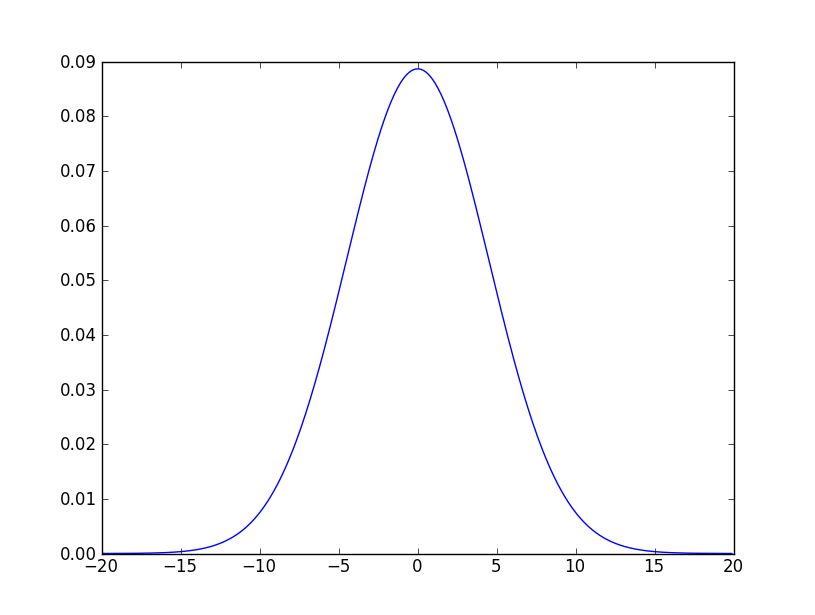
\includegraphics[width=1\linewidth]{img/cylinderGauss.png} \\ а)}
	\end{minipage}
	\hfill
	\begin{minipage}[h]{0.49\linewidth}
		\center{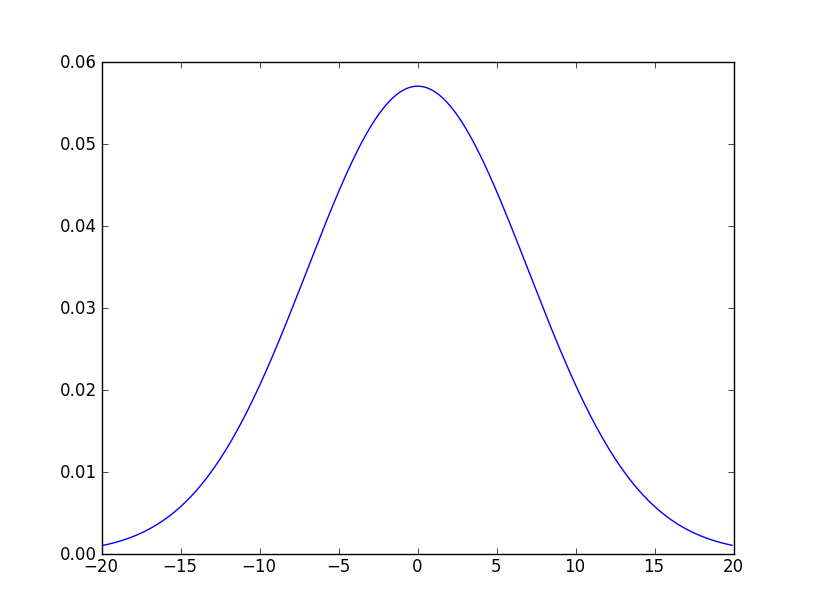
\includegraphics[width=1\linewidth]{img/planarGauss.png} \\ б)}
	\end{minipage}
	\caption{Распределение поля в волноводах: а) первый, б) второй}
	\label{diameter}
\end{figure}

Целью данной работы является рассмотрение эффективности передачи энергии при соединении волноводов. Опишем эту зависимость теоретически.

Из Лефевра известно, что отношение интенсивности $C$ это отношение скалярного квадрата мощности связанной волны к скалярному квадрату мощности входной волны. Его можно найти по формуле:

\begin{equation}
	\label{coupling_full}
	C = \frac{\left[\int\limits_{-\infty}^{\infty}E_{in}(x)e_{f0}^*(x) \,dx\right]^2}
	{\int\limits_{-\infty}^{\infty}e_{f0}(x)e_{f0}^*(x) \,dx
	 \int\limits_{-\infty}^{\infty}E_{in}(x)E_{in}^*(x) \,dx}
\end{equation}

Так как мы рассматриваем только действительную часть распределения, то формула упрощается:

\begin{equation}
	\label{coupling}
	C = \frac{\left[\int\limits_{-\infty}^{\infty}E_{in}(x)e_{f0}(x) \,dx\right]^2}
	{\int\limits_{-\infty}^{\infty}e_{f0}(x)^2 \,dx
	 \int\limits_{-\infty}^{\infty}E_{in}(x)^2 \,dx}
\end{equation}

Это выражение называется интегралом перекрытия  и показывает, какая часть энергии перейдет в возбуждение моды во втором волноводе. 

Эта величина максимальна и равна 1 при совпадении формы и центра каждого и уменьшается при увеличении расстояния между их центрами. Зафиксируем положение планарного волновода и будем перемещать центр цилиндрического, при этом будем вычислять значение интеграла (\ref{transition}). Воспользуемся для этого библиотекой scipy и языком программирования Python и получим график:
\begin{figure}[h!]
	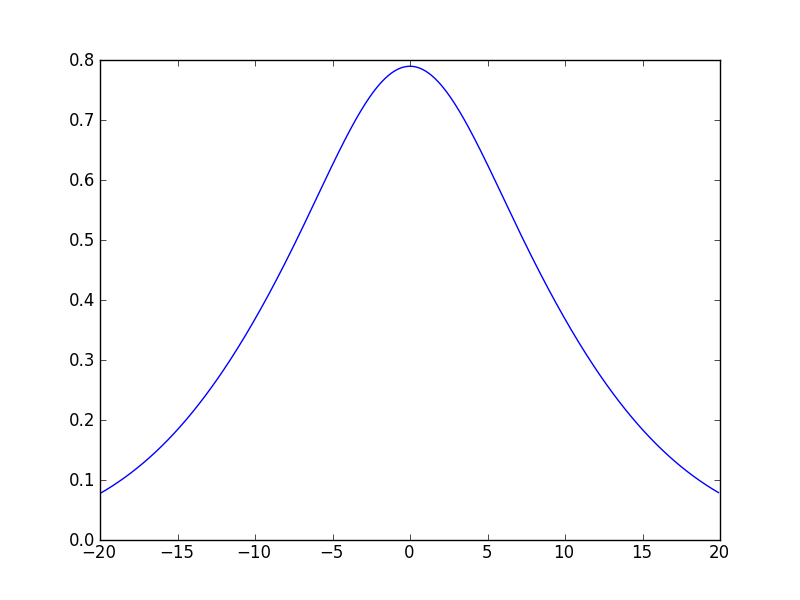
\includegraphics[width=0.5\textwidth]{img/transition.png}
	\caption{Зависимость к-та передачи от взаимного положения волноводов}
\end{figure}

\section{Поле волноводов в пространстве}

Выше рассматривался двухмерный случай распределения поля. В трехмерном случае нормальное распределение зависит от двух координат и равно:
\begin{equation}
  \label{gauss3d}
  E(x,y)=\frac{1}{2\pi\sigma_1\sigma_2}\exp\left(-\frac{x^2}{2\sigma_1^2}-\frac{y^2}{2\sigma_2^2}\right)
\end{equation}
где $\sigma_1$ и $\sigma_2$ - радиус моды по осям $x$ и $y$ соответственно. График этого уравнения выглядит представлен на рисунке \ref{gauss3dPlot}.

Аналогично двухмерному случаю, найдем интеграл перекрытия.

\begin{equation}
	\label{coupling}
	C = \frac{\left[\iint\limits_{-\infty}^{\infty}E_{in}(x,y)e_{f0}(x,y) \,dxdy\right]^2}
	{\iint\limits_{-\infty}^{\infty}e_{f0}(x,y)^2 \,dxdy
	 \iint\limits_{-\infty}^{\infty}E_{in}(x,y)^2 \,dxdy}
\end{equation}

\begin{figure}[h!]
	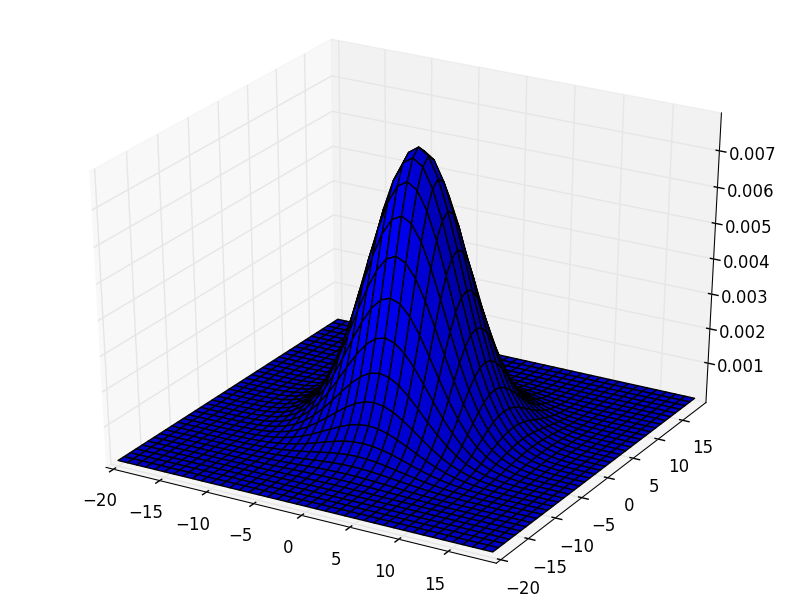
\includegraphics[width=0.5\textwidth]{img/gauss3d.png}
	\caption{Распределение Гаусса в пространстве}
	\label{gauss3dPlot}
\end{figure}


\chapter{Моделирование}
\section{Инструменты моделирования}
Для нахождения позиции оптимального совмещения волноводов, необходимо смоделировать поле волновода, и вычислить интеграл перекрытия, формула которого приведена в главе \ref{coupling}. Перебирая варианты взаимного расположения полей, необходимо найти максимальное значение этого интеграла.

Перебор всех теоретически возможных вариантов занимает длительное время, поэтому стоит его упростить, предполагая единственный максимум у функции. Для оптимизации поиска экстремумов функции используют методы координатного спуска, градиентного (наискорейшего) спуска и симплекс-метод.\cite{numeric} 

Предполагая, что у искомого распределения значений интеграла перекрытия имеется только один максимум, используем метод градиентного спуска, поскольку в этом случае он позволит достичь результата за меньшее число итераций. \cite{mathews}

Итак, нам нужен инструмент, позволяющий считать интегралы, проводить итерации и строить графики. В работе используется язык программирования Python, имеющий все необходимое. 

Для решения наших задач, к Python подключаются следующие внешние библиотеки:
\begin{itemize}
	\item NumPy - пакет функций для базовых операций с матрицами (создание и итерация по ним)
	\item SciPy - пакет математических функций, используется для интегрирования и содержит реализацию алгоритма градиентного спуска
	\item Mathplotlib - для вывода полученных результатов в виде графиков.
\end{itemize}

Кроме того, функция распределения Гаусса, для повышения производительности программы, также была вынесена в отдельный модуль.

\section{Моделирование поперечного смещения}

При поперечном смещении центр выходного поля смещается относительно входного на расстояние $\Delta x$, как показано на рисунке \ref{transverse_movement}. Для исследования коэффициента передачи была написана программа, вычисляющая значения интеграла перекрытия в пределах $x \in [-20, 20]$.
Для моделирования использовались два случая
\begin{itemize}
	\item Два одинаковых цилиндрических волновода с радиусом моды 4~мкм
	\item Два разных цилиндрических волновода с радиусами моды 4~мкм и 7~мкм соответственно
\end{itemize}

\begin{figure}[h!]
		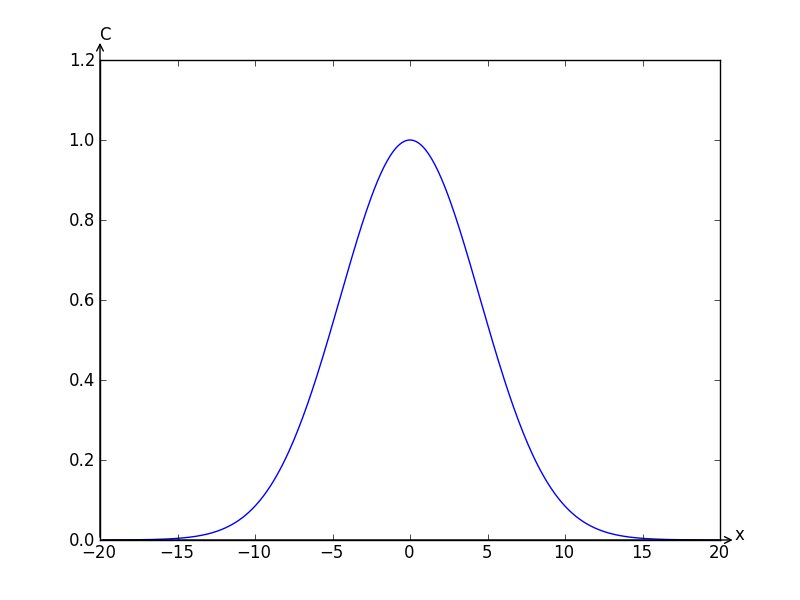
\includegraphics[width=0.5\linewidth]{img/twoCylinders.png}
		\caption{Зависимость коэффициента передачи двух одинаковых волноводов с радиусом моды 4~мкм}
\end{figure}
\begin{figure}[h!]
		\includegraphics[width=0.5\linewidth]{img/twoCylinders2.png}
		\caption{Зависимость коэффициента передачи двух волноводов с радиусами моды 4~мкм и 7~мкм}
		\label{twoCylinders2}
\end{figure}

В ходе моделирования, было обнаружено, что только два одинаковых волновода теоретически позволяют достичь стыковки без потерь. Во втором случае, показанном на рисунке \ref{twoCylinders2} максимальное значение составило 0.862 и это значение будет уменьшаться с ростом разницы в размерах волноводов.

\section{Моделирование продольного смещения}
При продольном смещении необходимо решить задачу нахождения вида пучка на некотором расстоянии от выхода волновода, после чего подставить получившееся распределение в интеграл перекрытия (\ref{coupling}) и определить эффективность передачи.
В моделировании будем использовать планарный волновод, описанный в \ref{strip_field} и цилиндрический с радиусом моды 3~мкм по обеим осям и показателем преломления сердцевины $n$ = 1.47. Длину волны лучей примем $\lambda$ = 1.55~мкм

\begin{figure}[h!]
	\includegraphics[width=0.5\linewidth]{img/longitudinal.png}
	\caption{Коэффициент передачи в зависимости от расстояния между волноводами}
	\label{longitudinal}
\end{figure}

\section{Интерактивная модель}
Для решения основной задачи, то есть поиска точки контакта с максимальным значением коэффициента передачи, была построена отдельная программа.

В ней слева показывается поле в выходном волноводе, а справа - схематическое расположение перекрывающихся полей. Ниже показаны числовые значения рассчитываемых параметров. Изначально программа позиционирует волноводы так, чтобы коэффициент передачи был максимален. Кликами по распределению поля можно виртуально изменять положение выходного волновода относительно входного и изображение будет перестраиваться, показывая новое распределение. Таким образом, можно наблюдать что произойдет при отклонении от точки максимального контакта.

\begin{figure}[h!]
	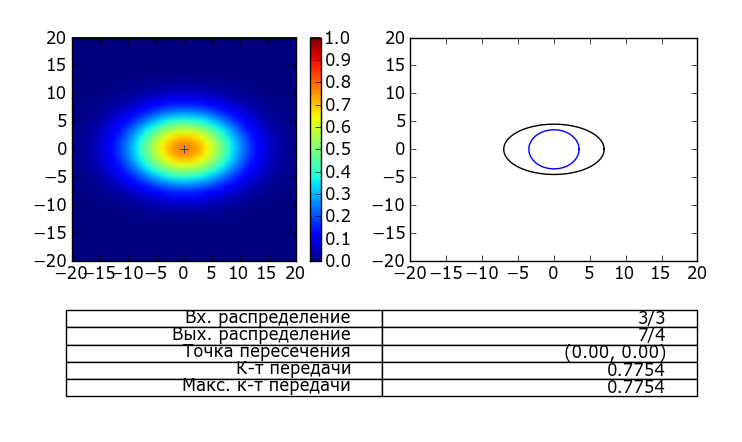
\includegraphics[width=\linewidth]{img/heatmap.png}
	\caption{Общий вид программы}
\end{figure}
\chapter{Технико-экономический анализ расчета эффективности связи двух волноводов}
\section{Выбор аналога объекта разработки}
Аналог объекта разработки — это объект, с аналогичным  функциональным назначением и являющийся  на данный момент времени лучшим по своим технико-эксплуатационным характеристикам.
Проведенный патентный и литературный, а также поиск в сети Интернет показали, что программные средства, обеспечивающие расчет эффективности связи мод двух волноводов, являются закрытыми.

\section{Определение товарного типа объекта разработки}
Товарный тип объекта разработки устанавливается путем анализа рыночной цели его создания. С этой точки зрения выделяются следующие типы:
\begin{itemize}
	\item разработки, выполняемые с коммерческой целью, то есть предназначенные для реализации на рынке. Общей характерной чертой  таких разработок является более или менее широкий спрос на их результаты на рынке (наличие нескольких потребителей). Такие разработки могут быть двух типов: имеющие рыночный аналог и не имеющие  рыночного аналога. Аналогом объекта разработки считается объект, имеющий аналогичное функциональное назначение и являющийся лучшим по своим технико-эксплуатационным характеристикам на данный момент времени.
	\item разработки, выполняемые с некоммерческой целью, то есть не предназначенные для прямой или косвенной реализации на рынке.
\end{itemize}
Целью данной дипломной работы является разработка программы, предназначенной для расчета эффективности связи мод двух волноводов. Эта разработка выполнялась с некоммерческой целью, то есть не была предназначена для прямой или косвенной реализации на рынке.
Согласно классификации, объект разработки относится к последнему типу (разработки, выполняемые с некоммерческой целью) \cite{economics}. Отнесение объекта разработки к определенному товарному типу определяет необходимые дальнейшие расчеты в экономической части. В данном случае в экономический расчет составит только смета затрат на разработку по методу сметного калькулирования.

\section{Расчет сметы затрат на разработку}
В состав сметной стоимости разработки входят следующие статьи затрат:
\begin{itemize}
\item материалы, покупные изделия и полуфабрикаты;
\item специальное оборудование для проведения разработки;
\item основная заработная плата разработчиков;
\item дополнительная заработная плата;
\item отчисления в социальные внебюджетные фонды;
\item затраты на электроэнергию для технологических целей;
\item затраты на командировки;
\item контрагентские работы;
\item прочие затраты;
\item накладные расходы.
\end{itemize}
Сметная стоимость определяется методом сметного калькулирования, то есть определением затрат по отдельным статьям и последующим суммированием.

\subsection{Расчет затрат на комплектующие изделия и полуфабрикаты}
Для создания данного продукта не использовались расходные материалы и покупные изделия, поскольку он является результатом умственного труда, поэтому затраты на комплектующие отсутствуют.

\subsection{Расчет затрат на основную заработную плату}
Основная заработная плата сотрудников ($C_oc$) определяется по формуле \ref{zarplat}: 
\begin{equation}
	C_{oc} = \sum_{j=1}^k \textit{П}_{mj} \cdot \overline{\textit{З}_{mj}} \cdot P \mbox{, (руб.)}
	\label{zarplat}
\end{equation}
где  $k$ – количество категорий разработчиков;\\
$\textit{П}_{mj}$ – количество разработчиков данной категории;\\
$\overline{\textit{З}_{mj}}$ - среднечасовая заработная плата j-категории разработчиков, руб/час;\\
$P$ – продолжительность работы, выполняемой работником определенной категории, час.

В разработке и реализации данного проекта участвовали 2 две категории разработчиков: руководитель и один инженер-разработчик.

Среднечасовая заработная плата руководителя рассчитывается с учетом того, что его среднемесячная заработная плата составляет 40\,000 рублей. Если рабочий день принять восьмичасовым, а количество рабочих дней в месяце~--~22, то его среднечасовая заработная плата составит:
$$
	\textit{З}_{m1} = \frac{40\,000}{8 \cdot 22} = 227.27 \mbox{ руб/час}
$$
Среднемесячная заработная плата инженера-разработчика составляет 35\,000 рублей. Отсюда можно найти его среднечасовую заработную плату. Если рабочий день принять восьмичасовым, а количество рабочих дней в месяце~--~22, то его среднечасовая заработная плата составит:
$$
	\textit{З}_{m1} = \frac{35\,000}{8 \cdot 22} = 198.86 \mbox{ руб/час}
$$
Общее время затраченное на разработку программного обеспечения составит:
$$
	P = 4 \cdot 22 \cdot 8 = 704 \textsc{ час}.
$$
Основная заработная плата работников рассчитана в таблице \ref{zp_table}:

\begin{table}[h]
	\caption{Основная заработная плата работников}
	\label{zp_table}
	\begin{tabular}{|l|l|l|l|}
		\hline
			Сотрудник & \thead{Среднечасовая\\ заработная плата,\\руб./час} & \thead{Время\\работы,\\час} & \thead{Основная\\заработная плата,\\руб.}\\
		\hline
			Руководитель & 227.27 & 704 & 159\,998 \\
		\hline
			Инженер & 198.86 & 704 & 139\,997 \\
		\hline			
			Итого: & & & 299\,995 \\
		\hline					
	\end{tabular}
\end{table}

\subsection{Расчет дополнительной заработной платы сотрудников}
Дополнительная заработная плата сотрудников, проводящих разработку ($C_\textit{доп}$) определяется по формуле \ref{zarplat_ext}:
\begin{equation}
	C_\textit{доп} = \frac{C_{oc} \cdot d}{100} \mbox{, (руб.)}
	\label{zarplat_ext}
\end{equation}  

где $d$ – норматив затрат на дополнительную зарплату от основной, $d=10\%$.
$$
	C_\textit{доп}  = 299\,995 \cdot 0.10 = 29\,999.5 \mbox{ руб.}
$$

\subsection{Расчет затрат на отчисления в социальные внебюджетные фонды}
Отчисления в социальные внебюджетные фонды определяются по формуле \ref{zarplat_fonds}

\begin{equation}
	C_\textit{сф} = \frac{(C_{oc} + C_\textit{доп}) \cdot r}{100} \mbox{, (руб.)}
	\label{zarplat_fonds}
\end{equation} 
где $r$ – суммарная величина единого социального налога  и отчисления на страхование от несчастных случаев. По состоянию на 01.01.2013: $r = 22.0\%	+ 2.9\% + 5.1\% = 30\%$.
$$
	C_\textit{сф} = (299\,995 + 29\,999.5)\cdot 0.3 = 98\,998 \mbox{ руб.}
$$

\subsection{Расчет затрат на технологическое топливо и электроэнергию}
Затраты на электроэнергию для технологических целей определяются по формуле \ref{electricity}:
\begin{equation}
	C_\textit{эн} = \sum_{i=1}^l W_i \cdot T_i \cdot C_{kr} \cdot K_{wi} \mbox{, (руб.)}
	\label{electricity}
\end{equation}

где  $l$ – номенклатура оборудования, используемого для разработки;\\
$W_i$ – мощность оборудования по паспорту, кВт;\\
$T_i$ – время использования для проведения разработки, час;\\
$C_{kr}$ – стоимость одного кВт\textperiodcentered час электроэнергии, руб;\\
$K_{wi}$ – коэффициент использования мощности ($K_{wi} < 1$).\\

\begin{table}[h]
	\caption{Затраты на электроэнергию для технологических целей}
	\begin{tabular}{|l|l|l|l|l|l|}
		\hline
			Оборудование & \thead{Мощность\\ по паспорту,\\кВт} & \thead{Время\\использования,\\час} & \thead{Коэффициент\\использования} & \thead{Стоимость\\одного\\кВт-час, руб} &  \thead{Затраты,\\руб} \\
		\hline
			ЭВМ & 0.4 & 704 & 0.95 & 3 & 802.56 \\
		\hline
			Итого: & & & & & 802.56 \\
		\hline		
	\end{tabular}
\end{table}

\subsection{Расчет затрат на командировки}
Затраты на командировки не производились.

\subsection{Расчет затрат на контрагентские работы}
Контрагентские работы ($C_\textit{кр}$) не проводились

\subsection{Расчет прочих затрат}
К статье <<прочие затраты>> ($C_\textit{п}$) относятся затраты, связанные с оплатой экспертиз, консультаций, получения патентной информации, арендой помещения, и затраты на канцелярские товары и т.д. Эти затраты задаются в процентах к суммарной величине предыдущих статей ($10\%$) по формуле \ref{cost_other}
\begin{equation}
	C_\textit{п} = (C_\textit{м}+C_\textit{об}+C_\textit{ос}+C_\textit{доп}+C_\textit{сф}+ C_\textit{эн}+C_\textit{кр})\cdot r \mbox{, (руб.)}
	\label{cost_other}
\end{equation}
где $r=10\%$.
$$
	C_\textit{П} = (299\,995 + 29\,999 + 98\,998 + 802.56)\cdot 0.1 = 43\,309 \mbox{ руб.}
$$

\subsection{Расчет накладных расходов}
Накладные расходы ($C_\textit{н}$) определяются по формуле \ref{cost_util}, где $r = 80\%$:
\begin{equation}
	C_\textit{н} = C_\textit{ос} \cdot r \mbox{, (руб.)}
	\label{cost_util}
\end{equation}
$$
	C_\textit{н} = 299\,995 \cdot 0.8 = 239\,996 \mbox{ руб.}
$$

\subsection{Расчет общей сметной стоимости}
Итак, найдем общую сметную стоимость разработки. Общая сметная стоимость ($C_\textit{р}$) определяется сложением ее составляющих:
\begin{equation}
	C_\textit{р} = C_\textit{м}+C_\textit{об}+C_\textit{ос}+C_\textit{доп}+C_\textit{сф}+ C_\textit{эн}+C_\textit{кр}+C_\textit{п}+C_\textit{н} \mbox{, (руб.)}
\end{equation}

Общая стоимость разработки и ее составляющие части приведены в таблице \ref{cost_total}.

\begin{table}[h!]
	\caption{Сметная стоимость проведения разработки}
	\label{cost_total}
	\begin{tabular}{|c|p{9cm}|c|c|}
		\hline
			\thead{\No \\ п/п} & Статьи расходов & \thead{Условные\\обозначения} & \thead{Затраты по\\ статьям, руб.}\\
		\hline
			1 & Основная заработная плата & $C_\textit{ос}$ & 299\,995 \\
		\hline
			2 & Дополнительная заработная плата & $C_\textit{доп}$ & 29\,999.5 \\
		\hline
			3 & Отчисления в социальные внебюджетные фонды & $C_\textit{сф}$ & 98\,998 \\
		\hline
			4 & Затраты на электроэнергию для технологических целей  & $C_\textit{сф}$ & 802.56 \\
		\hline
			5 & Прочие прямые затраты & $C_\textit{п}$ & 42\,980 \\
		\hline		
			6 & Накладные расходы & $C_\textit{н}$ & 239\,996 \\
		\hline		
			\multicolumn{2}{|l|}{Общая сметная стоимость} & $C_\textit{р}$ & 712\,771 \\
		\hline
	\end{tabular}
\end{table}
\chapter{Безопасность жизнедеятельности}
\section*{Заключение}
\addcontentsline{toc}{chapter}{Заключение}

В результате проведенной выпускной квалификационной работы был разработан метод расчета эффективности связи двух волноводов с помощью интеграла перекрытия.
\bibliography{../lib}
\addcontentsline{toc}{chapter}{Литература}
\end{document}